% id: 94-34
% book: 쎈B 대수 · 07 삼각함수의 활용
% section: 유형 08 사인법칙과 코사인법칙
% figure: tikz:fig-94-34
% answer: 
% answer_source: 
% variant_level: 0 (원본 전사)
% 이 파일은 build.mjs 가 items.json 에서 만든다. 고칠 때는 items.json 을 고친다.
\smash{\raisebox{1.5mm}{\dmkichul{서술형}}}
아래 그림에서 삼각형~$\pt{ABC}$의 변 $\pt{BC}$ 위의 점~$\pt{D}$가 다음 조건을 모두 만족시킬 때, $\sin C$의 값을 구하시오. \exprbox{\begin{minipage}{0.96\linewidth}\raggedright ㈎ $\seg{AB}=\seg{BD}=\dfrac{2}{3}\seg{AD}$\\[2.5mm] ㈏ $\seg{AC}=2\seg{AD}$\end{minipage}}
\par\smallskip\begin{center}\resizebox{\ifdim\width>\linewidth\linewidth\else\width\fi}{!}{% 94-34(94쪽) — 변 $\pt{BC}$ 위의 점 $\pt{D}$ 가 있는 삼각형 $\pt{ABC}$(원문 「아래 그림」). 스캔 화질이 낮아 TikZ 로 다시 그림.
% 라벨은 원문 것만: 꼭짓점 $\pt{A}$·$\pt{B}$·$\pt{C}$·$\pt{D}$ 뿐이다. 조건 (가)(나)의 길이는 본문에만 있으므로 그림에 적지 않는다.
% $\sin C$ 의 값(답)이 읽히지 않게 각·눈금은 그리지 않는다.
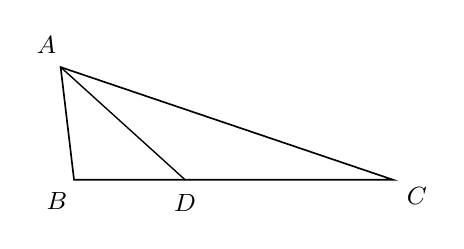
\begin{tikzpicture}[line width=0.6pt]
  \draw (-0.17,1.43) -- (0,0) -- (4.05,0) -- cycle;
  \draw[line width=0.5pt] (-0.17,1.43) -- (1.41,0);
  \node[anchor=south east, font=\small] at (-0.10,1.47) {$\pt{A}$};
  \node[anchor=north east, font=\small] at (0.04,-0.03) {$\pt{B}$};
  \node[anchor=north west, font=\small] at (4.10,0.03) {$\pt{C}$};
  \node[anchor=north, font=\small] at (1.41,-0.06) {$\pt{D}$};
\end{tikzpicture}
}\end{center}
